\chapter{Methodiek van de testen}	
Dit hoofdstuk behandelt de wijze waarop de testen naar consistentie, failure handling en recovery worden uitgevoerd. 
De methodiek kan opgedeeld worden in 4 grote stappen: het opstellen, kalibreren, testen van de systemen en tenslotte het verzamelen en analyseren van de resultaten.

\paragraph{Opstellen van de testomgeving} Deze eerste stap is voor het installeren en configureren van de DBMS en de testsoftware. Een variatie in hardware van de systemen, versienummer van de software of een verschillende netwerkinfrastructuur kunnen de uiteindelijke testresultaten beïnvloeden. 

\paragraph{Calibratie van de testomgeving} In de uiteindelijke testen wordt het gedrag onder normale belasting getest. Afhankelijk van de gekozen systemen, netwerkinfrastructuur zal dit voor elke DBMS een verschillende belasting geven. Deze stap bepaalt hoeveel gebruikers er zijn in het systeem en hoeveel bewerkingen er uitgevoerd worden per second. 

\paragraph{Testen van de systemen} In deze stap worden de testen op de verschillende systemen uitgevoerd. Voor deze methodiek is het mogelijk om te testen hoe de latency van een bewerken zich gedraagt voor, tijdens en na het falen en herstellen van een systeem.  Daarnaast is er ook een testmethode voor een actieve analyse van eventuele consistentie. 

\paragraph{Verzamelen en analyseren van de testdata} In de laatste stap wordt de data van de vorige stappen verzameld en de resultaten worden visueel voorgesteld. Met behulp van de uitgebreide testdata, is het ook mogelijk om bepaalde conclusies te maken over een passieve analyse van eventuele consistentie. 

In de volgende secties komen de verschillende stappen in meer detail aanbod.  Een overzicht van de procedure kan gevonden worden in figuur \ref{fig:test-process-overview}
\begin{figure}[h!]
\centering
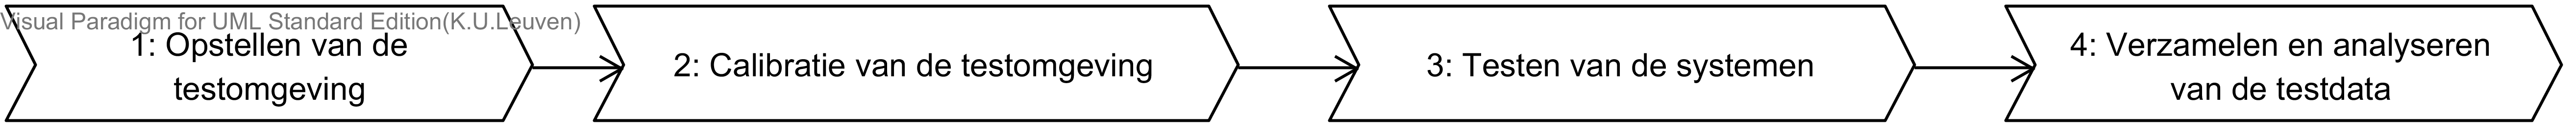
\includegraphics[width=\linewidth]{img/Test-Process-Overview}
\caption{Overzicht testproces}
\label{fig:test-process-overview}
\end{figure}

\section{Stap 1: Opstellen van de testomgeving}
Het installeren en configureren een softwarepakket op een enkel systeem, is in Unix systemen veelvuldig geautomatiseerd met behulp van tools zoals \gls{apt-get} en \gls{yum}. Voor een systeem in een gedistribueerde omgeving, is de situatie iets ingewikkelder. Naast de lokale installatie en configuratie, is er ook een gedistribueerde configuratie stap.  

In deze gedistribueerde configuratie stap, worden de verschillende systemen van elkaars bestaan op de hoogte gebracht, hiervoor bestaan twee verschillende methodes maar ook een combinatie van de configuratie methodes is mogelijk.
 
\paragraph{Configuratie bestanden} Met deze methode dient er op elke lokaal systeem een configuratiebestand aangemaakt of aangepast worden met hierin één of meerdere andere leden. Nadien kunnen de verschillende lokale systemen opgestart worden of de configuratiebestanden worden opnieuw ingeladen in de al draaiende systemen. Vervolgens zullen met de configuratie elkaar vinden en samen het database systeem vormen. Deze informatie kan een ip adres zijn van één of meerdere systemen maar dit kan ook een naam zijn van het systeem die met een broadcast verdeeld wordt. 
\paragraph{Centrale configuratie} Bij een centrale configuratie, worden de systemen lokaal opgestart zonder enige lokale configuratie. Vervolgens wordt via een console, webinterface, ... connectie gemaakt met een node. Deze krijgt configuratie informatie hoe deze zich moet gedragen en volgt deze informatie op. In deze systemen is de configuratie tijdens installatie gelijk en wordt de configuratie verspreid wanneer de systemen al draaien.  


Deze stap is gelijk aan het opzetten van het systeem in een productie omgeving, na het uitvoeren van deze stap, zou het DBMS immers succesvol moeten werken. 

\section{Stap 2: Calibratie van de testomgeving}
Afhankelijk van de onderliggende infrastructuur en het soort DBMS, kan het systeem een verschillend gedrag hebben onder dezelfde configuratie. Voor de eigenlijk testen is het de bedoeling om een middelmatige belasting te hebben. De queuing theory geeft de eigenschap dat $R = S + W$ waar R de totale vertraging is, S de processing time en W de tijd in de wachtrij \cite{millsap2003optimizing}\todo{Betere referentie dan Oracle?}. Dit verband is visueel voorgesteld ten opzichte van de belasting in figuur \ref{fig:hockey-stick}. 

\begin{figure}[h!] 
\centering
	\subfigure[Verband vertraging ten opzicht van de belasting van een DBMS.]{\label{fig:hockey-stick} 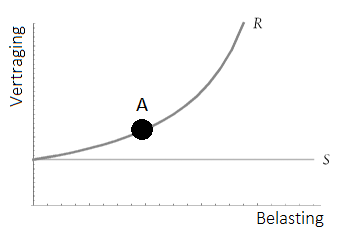
\includegraphics[width=0.45\textwidth]{img/hockey-stick}}
	\hfill
	\subfigure[Verband vertraging ten opzicht van het aantal gebruikers.]{\label{fig:connecties-gebruikers} 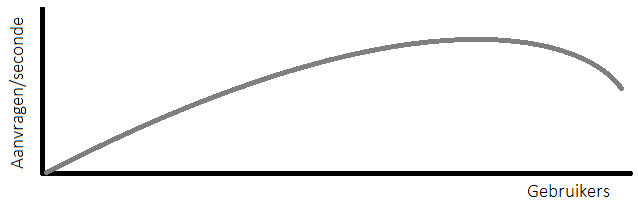
\includegraphics[width=0.45\textwidth]{img/connecties-gebruikers}}
	\caption{}
\end{figure}
\todo{Vind er betere ;-) }
Deze belasting kan afhankelijk zijn verschillende elementen, er worden 5 verschillende mogelijke parameter groepen besproken:

\paragraph{Hoeveelheid data per gegevensrecord} Elke record in de database kan bestaan uit verschillende kolommen en per kolom een waarde. Het is belangrijk om te definiëren hoe groot een gemiddeld record is, aangezien dit een invloed heeft op het schijfgebruik en het netwerkverkeer.   

\paragraph{Type van queries} De opgeslagen data kan opgevraagd worden op verschillende wijze: data kan ingevoegd, aangepast, opgevraagd of verwijderd worden. Daarnaast kan dit gebeuren voor 1 of meerdere records tegelijk. Afhankelijk van de relatieve verhouding van deze soorten, kan een ander resultaat bekomen worden: sommige DBMS's zijn meer geschikt voor veelvuldig lezen dan schrijven en vice versa. 

\paragraph{Query specificatie} Bij het opvragen of verwijderen van een record, kan er een verschil zijn naar processing tijd afhankelijk van hoe lang geleden de record geschreven is en of naburige data onlangs gelezen is. Vandaar dat ook het datadistributie gekozen moet worden. Voorbeelden van verschillende technieken zijn: voornamelijk de laatste data lezen, een uniforme kans voor alle data of bepaalde records regelmatig lezen.

\paragraph{Aantal connecties of gebruikers} In een gedistribueerde omgeving zullen meestal meerdere gebruikers tegelijk actief zijn, maar sommige systemen hebben een voorkeur naar weinig connecties met grote hoeveelheden data, andere kunnen meer gebruikers tegelijk behandelen. Het totaal aantal queries kan berekend worden als: $\#Queries = \#Gebruikers * \#QueriesPerGebruiker$. In deze stap wordt er verondersteld dat de gebruiker het maximaal aantal queries doet, dus $1/Vertraging$. Rekening houdend met de exponentiële groei van de wachtrij vertraging (figuur \ref{fig:hockey-stick}), betekent dit dat er een totaal maximum aantal queries per seconde bereikt wordt bij een bepaald aantal gebruikers. In deze stap wordt er gezocht naar dit aantal gebruikers, zie figuur \ref{fig:connecties-gebruikers}. 

\paragraph{Aantal queries per seconde} In de vorige stap is er de optimale configuratie bepaald om het systeem maximaal te belasten. Maar in het begin is er gesteld dat er gezocht wordt naar een gemiddelde belasting voor dit aantal gebruikers. Er wordt gekozen om matige belasting, in figuur \ref{fig:hockey-stick} zou dit punt A zijn. 

Met de parameters afkomstig uit de calibratie, kunnen de testen opgestart en uitgevoerd worden. 

\section{Stap 3: Testen van de systemen}
In deze thesis zullen er 2 verschillende soort testen uitgevoerd worden, de beschikbaarheid en consistentie testen, welke beide dezelfde algemene stappen volgen, elk met hun eigen specifieke parameters. Er zijn de 6 deelstappen: 

\paragraph{Opstellen van de database} In stap 2 was er gekozen voor een bepaalde datastructuur, deze structuur wordt zo goed mogelijk meegegeven aan de DBMS zodat deze optimale allocatie kan doen.

\paragraph{Inladen van de data} Een bepaalde hoeveel data wordt vooraf ingeladen. Dit wordt gedaan om een basis dataset te hebben die nodig is voor sharding, het opsplitsen van de data over verschillende servers. In bepaalde DBMS's wordt dit automatisch toegepast, maar enkel bij een bepaald hoeveelheid data. Dit gebeurt op maximale snelheid. 

\paragraph{Pauze} Na het inladen van de data wordt enige tijd gewacht. Zoals aangetoond in YCSB++\cite[Figuur 9]{patil2011ycsb++}, is er hogere vertraging in de DBMS's onmiddellijk na het inlezen. Dit kan onder andere te wijten zijn doordat data nog weggeschreven moet worden naar schijf of in bepaalde systemen zou het kunnen dat de sharding gebeurt op momenten met weinig belasting. Om deze piek niet te hebben, wordt er enige tijd gewacht. 

\paragraph{Opstarten van de test (opstart kost)} De test wordt opgestart en de begint te lopen. In veel gevallen is er in het begin een opwarmfase nodig omdat de vertraging net hoger of lager is als na enige tijd. Deze hogere tijd is onder andere te verklaren doordat de connectie opgezet moet worden en caches worden gevuld. Soms is deze lager doordat de schijf nog niet belast is of de er nog veel schrijfbuffers leeg zijn. Om dit gedrag te vermijden, start de data van de eigenlijke test pas na deze stap. 

\paragraph{Uitvoeren van de test} De eigenlijke test wordt uitgevoerd en de data wordt verzameld en opgeslagen. De details van de beide testen volgen achteraf. 

\paragraph{Terugbrengen naar beginstatus} Na het uitvoeren van de test, wordt het DBMS terug naar de beginstatus gebracht. Onder andere de database en de data wordt volledig verwijderd. Belangrijk in dit geval is het controleren of de data volledig verwijderd is, in bepaalde gevallen wordt er nog ergens een veiligheidskopie bijgehouden dat herstelt wordt bij een mogelijke volgende batch. 

De twee verschillende testmethodes zullen nu in meer detail behandeld worden. 
\subsection{Beschikbaarheidstest}
Bij de beschikbaarheidstest wordt er gekeken hoe het systeem reageert op tijdelijk (on)verachte onbeschikbaarheid van een deel van het systeem. In deze testen worden er 3 mogelijke manieren getest die de systemen onbeschikbaar terwijl er de basisbelasting die bepaald is in stap 2, op uitvoert. 

\paragraph{Zachte stop} De DMBS service wordt gevraagd om te stoppen. Op deze manier krijgt de service eerst een signaal dat deze moet stoppen en kan deze de andere waarschuwen. Achteraf wordt dezelfde service terug opgestart. Dit simuleert het gepland uitschakelen van een systeem. 

\paragraph{Harde stop} De DMBS service wordt onmiddellijk gestopt door het process te beëindigen. De service heeft geen tijd om de andere te waarschuwen. Achteraf wordt dezelfde service terug opgestart. Dit simuleert een crash van de service die pas na enige tijd opgemerkt wordt. 

\paragraph{Netwerk onderbreken} Al het netwerk verkeer wordt gedropt zonder enige waarschuwing. De service heeft geen tijd om de andere te waarschuwen én de zender krijgt geen onbereikbaar antwoord. Achteraf wordt het netwerk verkeer terug toegelaten. Dit simuleert een onderbroken internetverbinding of een onbereikbare server om eender welke andere reden.  

Een zelfde systeem kan sterk verschillend reageren op de verschillende situaties: waar de eerste situatie nog eenvoudig is te behandelen doordat men op de hoogte is, is de tweede situatie al moeilijker alhoewel men wel antwoord krijgt dat de service niet beschikbaar is bij het contacteren. De derde situatie is het moeilijkste te behandelen omdat men niet weet of de berichten naar de server niet aankomen of de antwoorden verloren gaan. 
 
\subsection{Consistentie test}
In de consistentie test wordt onderzocht welke consistentie de DBMS ondersteund. Zoals voordien besproken in deel \ref{sec:eventualconsistency}, bestaan er verschillende soorten. 

In deze testen is er gekozen om caching bij de gebruiker \textbf{uit te schakelen}, dit om de reden dat dit gedrag zeer onvoorspelbaar is en afhankelijk van andere acties van de lezer en schrijver. Een andere reden is dat eventueel consistentie alleen een probleem is voor data die onmiddellijk beschikbaar moet zijn, met andere woorden data die men niet mag cachen. Dit heeft als gevolg dat de belasting op de server hoger kan zijn. 

\paragraph{Beschrijving van de test} Deze test bestaat uit 3 soorten gebruikers: er is 1 gebruiker die data schrijft (=S), een aantal lezer (=L's) en tenslotte zijn er nog andere gebruikers die ervoor zorgen dat er samen met de andere gebruikers een belasting is zo dicht mogelijk bij de basisbelasting. 
Het is belangrijk dat er een exacte synchronisatie in tijd is tussen de verschillende gebruikers, dit om de geregistreerde tijdstippen te kunnen vergelijken.
\todo{figuur met een periode}

\subparagraph{Taak van de schrijver} De schrijver schrijft, zoals zijn naam voorspelt, voorafbepaalde data weg op vooraf vastgelegde momenten. Deze data kan een nieuw record of een update van een record zijn. Deze registreert op welk moment deze taak exact is gestart en hoe/wanneer deze is beëindigd.

\subparagraph{Taak van de lezer} De taak van een individuele lezer is om op vooraf vastgelegde momenten de data van de schrijven te gaan lezen. Dit wordt periodiek herhaald tot de data correct is gelezen of een bepaalde tijd is verstreken. Er kan ook beslist worden om ook als de data correct gelezen is, opnieuw te proberen. De lezer registreert elke keer deze gaat lezen op welk moment deze exact is gaan lezen en wat het resultaat van de actie is.  

\subparagraph{Het plannen van de lezers} Zoals voordien vermeldt gaat de schrijver op bepaalde momenten schrijven en de lezer herhaalt het lezen periodiek. Het doel van de lezers is om allereerst verbonden te zijn met verschillende servers en daarnaast meer testpogingen hebben op het lezen van de data. Om deze laatste redenen worden de starttijdstippen voor de data te lezen, gelijk gespreid tussen de verschillende lezers. 

\paragraph{Soorten eventuele consistentie} Met deze uitgevoerde testen en data kan aangetoond worden dat bepaalde systemen bepaalde eventuele consistentie vereisten niet volgen. Het is in veel gevallen niet mogelijk om te bewijzen dat deze het wel uitvoeren omdat een voorbeeld niet sluitend is, maar een tegenvoorbeeld wel. 

\subparagraph{Strikte consistentie} Een systeem is niet strikt consistent indien één van de lezers het nieuwe record of de update niet lezen \textit{indien de leesactie gestart is na het voltooien van de schrijfactie}. In bepaalde gevallen is zelfs mogelijk om deze garantie strikter te maken tot \textit{indien de leesactie \underline{voltooid} is na het voltooien van de schrijfactie}. 

\subparagraph{Read your own writes consistentie} Deze eventuele consistentie kan ontkracht worden indien een schrijver onmiddellijk na het voltooien zijn eigen data opvraagt en niet de nieuwe waarde leest. Dit kan enkel getest worden indien de DBMS het mogelijk maakt om met een gebruiker te verbinden naar meerdere servers.  In onze methode is dit niet geïmplementeerd omdat de data van de testen zonder dit al de mogelijkheid tot het maken van een conclusie.  

\subparagraph{Session consistentie} Aangezien er al conclusies getrokken kunnen worden over de vorige en deze nog een zwakkere eis heeft, is dit niet geïmplementeerd. Maar opnieuw kan dit ontkracht worden door met de zelfde connectie als de schrijver te lezen. 

\subparagraph{Casual consistentie} Deze test kan uitgevoerd worden de schrijver verschillende schrijfacties na elkaar te laten uitvoeren met tussendoor te zijn laatste actie te lezen. De lezer leest de records in dezelfde of omgekeerde volgorde. Indien deze data van een latere schrijfactie leest maar nog niet van een vroegere, is dit ongeldig. De eis kan strenger gemaakt worden door de schrijver tussendoor niet te laten lezen, dit zou andere resultaten kunnen hebben. Deze consistentie is in zijn totaal niet getest. 

\subparagraph{Monotonic Read consistentie} In deze test blijft de lezer continue opnieuw proberen om dezelfde data te lezen, eenmaal deze een nieuwe versie heeft gelezen zou deze nooit meer een oudere mogen lezen. 

Zoals duidelijk hierboven, biedt deze aanpak de mogelijkheid aan om naast een actieve ook een passieve analyse te doen op de data. 

\section{Stap 4: Verzamelen en analyseren van de testdata}
Na het uitvoeren van de testen, dient de informatie die verschillende schrijver en lezers hebben vergaart samen gebracht te worden. Vervolgens kan de informatie verwerkt worden te bepalen hoe lang het duurt voor de data overal consistent is (actieve analyse) of om  tegenvoorbeeld te zijn voor een bepaalde consistentie categorie (passieve analyse). De analyse kan gebeuren op basis van de besproken methodes hierboven. 

Tenslotte worden er in de testen nog grafieken gegenereerd van de aanwezige data, dit met de voor de hand liggende reden dat een figuur veel meer duidelijkheid brengt over de data dan duizenden getallen.  

\section{Conclusie}
Een overzicht van de test methode kan gevonden worden in figuur \ref{fig:test-process-detailed}. Deze testmethode geeft de mogelijkheid om in verschillende database systemen zowel de beschikbaarheid als de consistentie te testen op een gelijkaardige manier. 

\begin{figure}[h!]
\centering
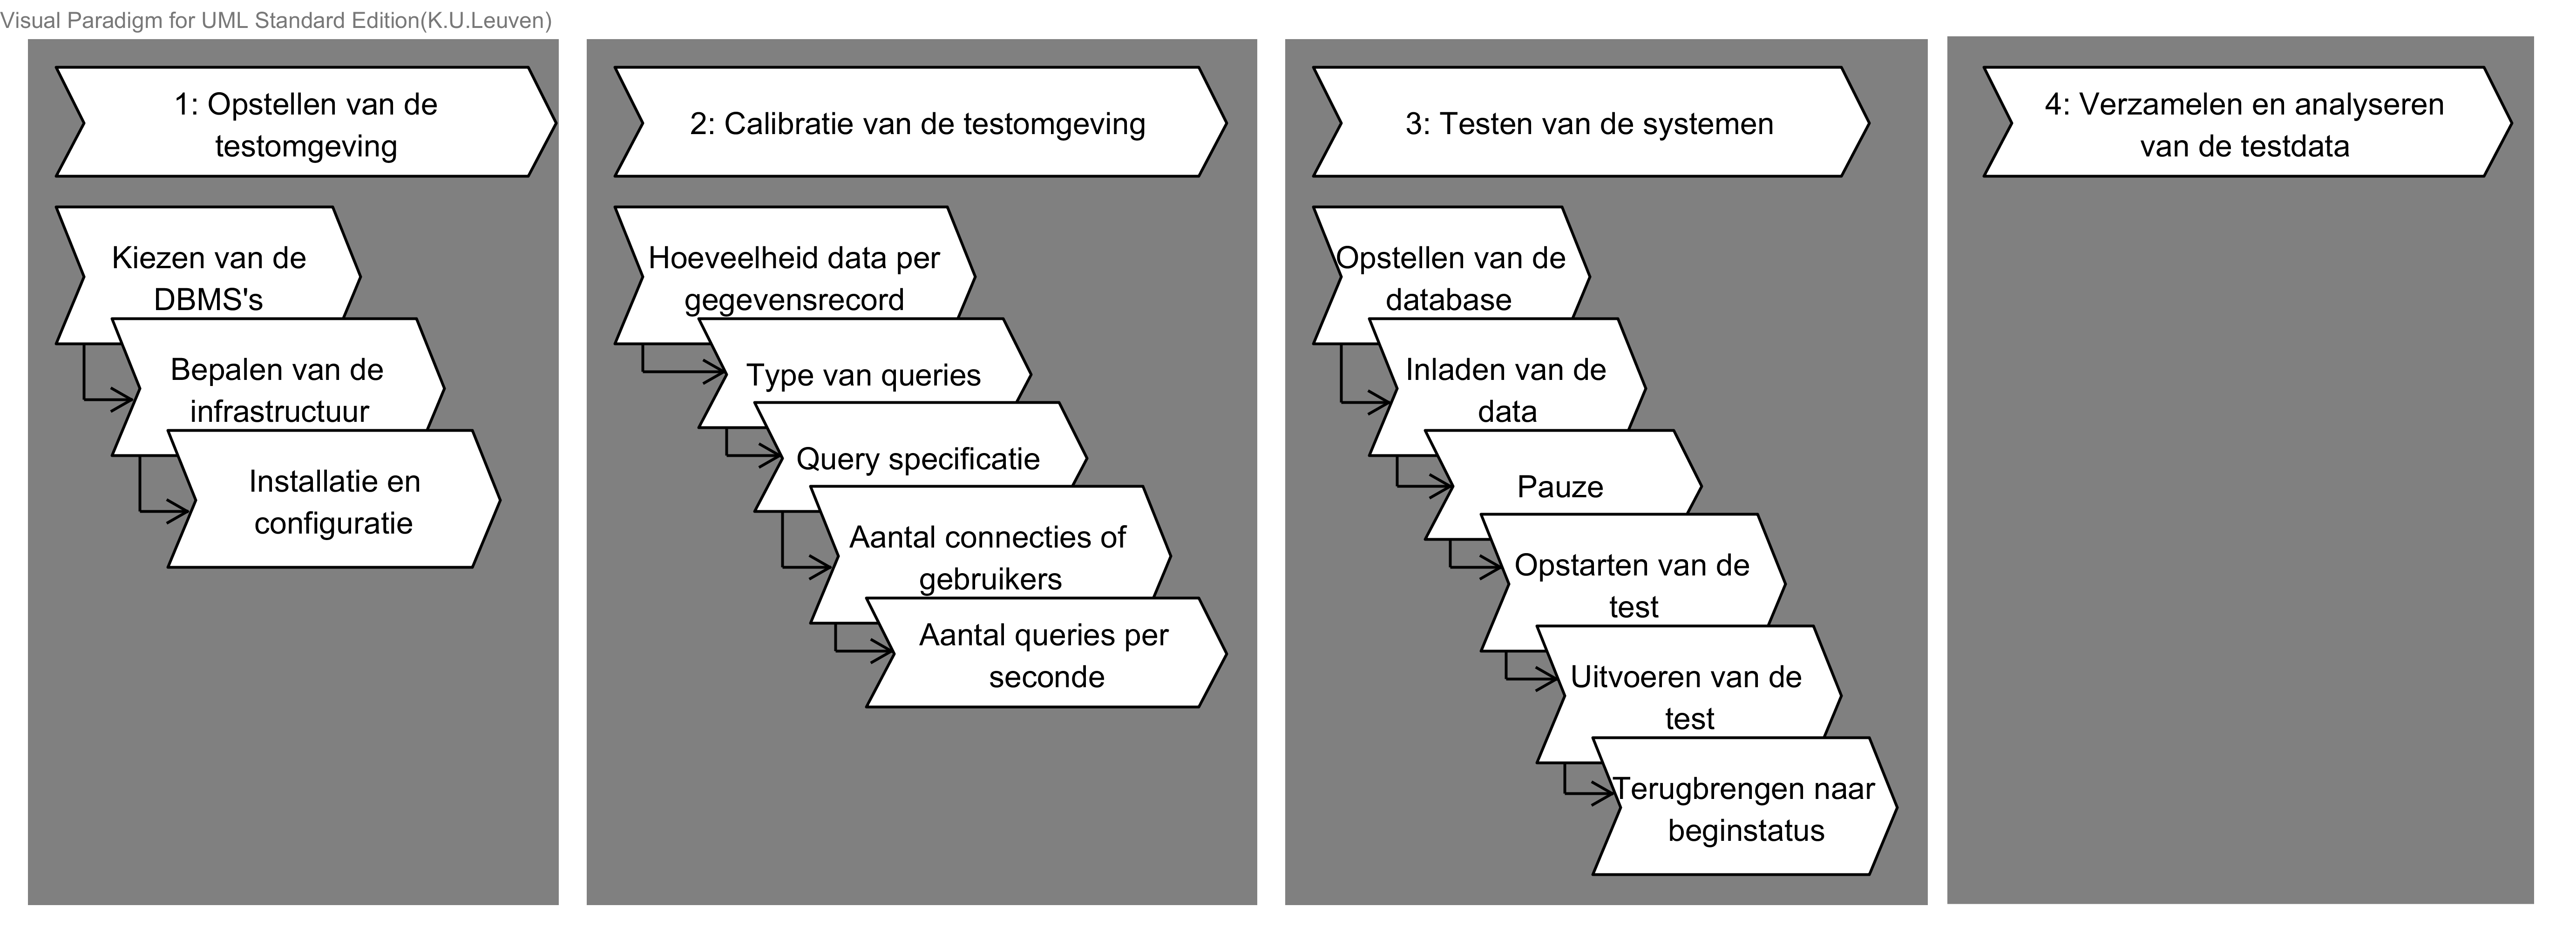
\includegraphics[width=\linewidth]{img/Test-Process-Detailed-Overview}
\caption{Overzicht testproces}
\label{fig:test-process-detailed}
\end{figure}
